%
\chapter{Architecture of distributed runtime monitoring}
%

As the needed source files are generated, we now can use them to execute the given graph queries on a distributed system. 
In the previous chapters, we could see how the framework generates the source codes, in this framework I show, how those source codes work



\section{Live model manipulation}
Model code is generated to help the creation and maintenance of the live model.
To create the model, first the \texttt{ModelRoot} class must be instantiated.
On different computation units, the models are synchronized over DDS.
Topics are created for two types of model update:
\begin{itemize}
	\item Object creation/deletion -- We need the information because if a graph pattern refers to remote objects, we create proxy elements for them.  
	\item Reference creation/deletion (change) -- This is needed, because references can have opposites: For one reference change on another computing unit, we may need to alter (create/delete) its opposite reference on an object, that may be on this computation unit.
\end{itemize}

\begin{figure}[H]
	\begin{center}
		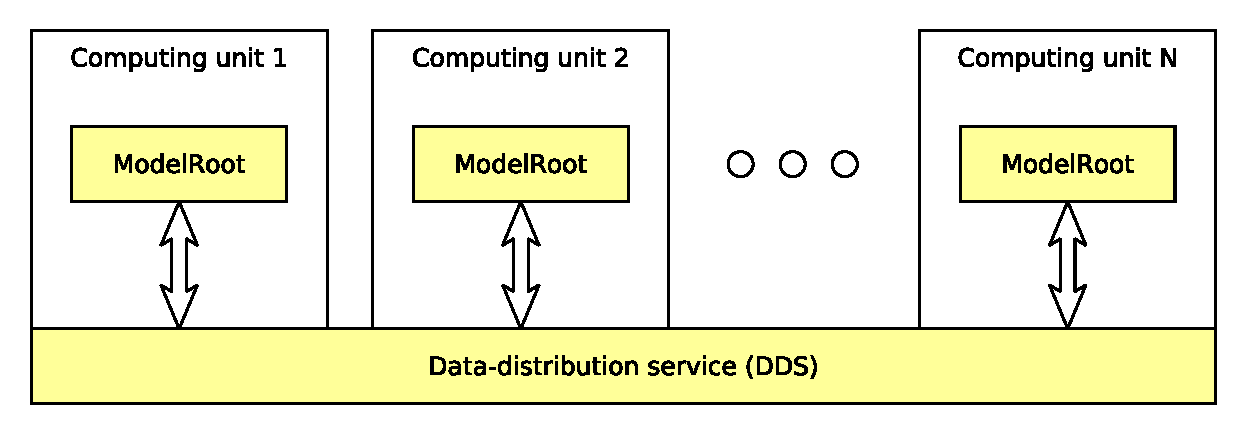
\includegraphics[width=0.8\textwidth]{figures/model-dds.pdf}
		\caption{ Synchronization of models via DDS }
		\label{fig:model-dds}
	\end{center}
\end{figure}

\section{Query execution}

The execution of the queries are happening at different computation units, which are connected via network.
On each computation unit, an instance of the software is running.
The basic architecture of the monitoring components of a running instance can be seen on \autoref{fig:query-runner-architecture}. \todo{be kell mutatni pontokba szedve, mi a feladata az egyes Query*-nak. Mikor, pontosan mit csinal, minek a hatasara. Egy peldan keresztul konkretan be lehetne mutatni, milyen Query* indul el, mit csinal, mikor all le, szerintem akkor lenne jol ertheto.}
The component called \texttt{QueryService} handles the communication between instances of the software.
\texttt{QueryRunner}s are responsible for running the local operations of a certain query execution. 
To achieve this, it uses the code generated by the framework.
Executing a query requires \texttt{QueryRunner}s on each computation unit assigned to each other and communicating via \texttt{QueryService}. 
Each \texttt{QueryRunner} processes the model while execute their search operations.

Query execution works the following way:
\begin{enumerate}
\item User invokes a query from a \texttt{QueryService}.
\item The \texttt{QueryService} requests the other instances of the software to create the appropiate query runners
\item Each \texttt{QueryService} creates a \texttt{QueryRunner} for the query
\item
\item
\end{enumerate}


\begin{figure}[H]
	\begin{center}
		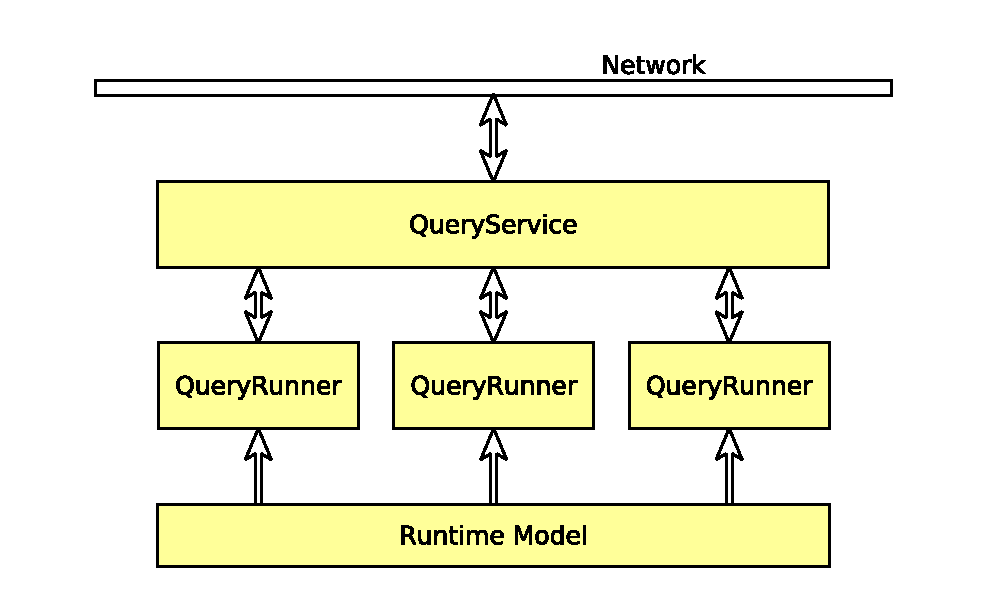
\includegraphics[width=0.8\textwidth]{figures/query-runner-architecture.pdf}
		\caption{ Basic architecture of the query running system }
		\label{fig:query-runner-architecture}
	\end{center}
\end{figure}









